\newpage

\chapter{My Notebook}

\section{Start importing}

\subsection{Some theory}
The Wasserstein Distance for 1D distributions can be obtained by:
\begin{displaymath}
	\int_0^1 |C_\alpha^{-1}(r) - C_\beta^{-1}(r)|^p dr \\
	\int_0^1 |C_\alpha^{-1}(r) - C_\beta^{-1}(r)|^p dr
\end{displaymath}
Where $C_\alpha^{-1}$ is the quantile function for the distribution $\alpha$ (the inverse of the Cumulative Distribution Function).Write some more markdown, with \textbf{bold text here} and \textit{italics} and \href{https://juliaoptimaltransport.github.io/OptimalTransport.jl/stable/examples/basic/}{a link here},another \textbf{bold} and \textit{more italics} and \href{https://github.com/}{another}. Ends with two figures
\begin{figure}[H]
	 \centering
	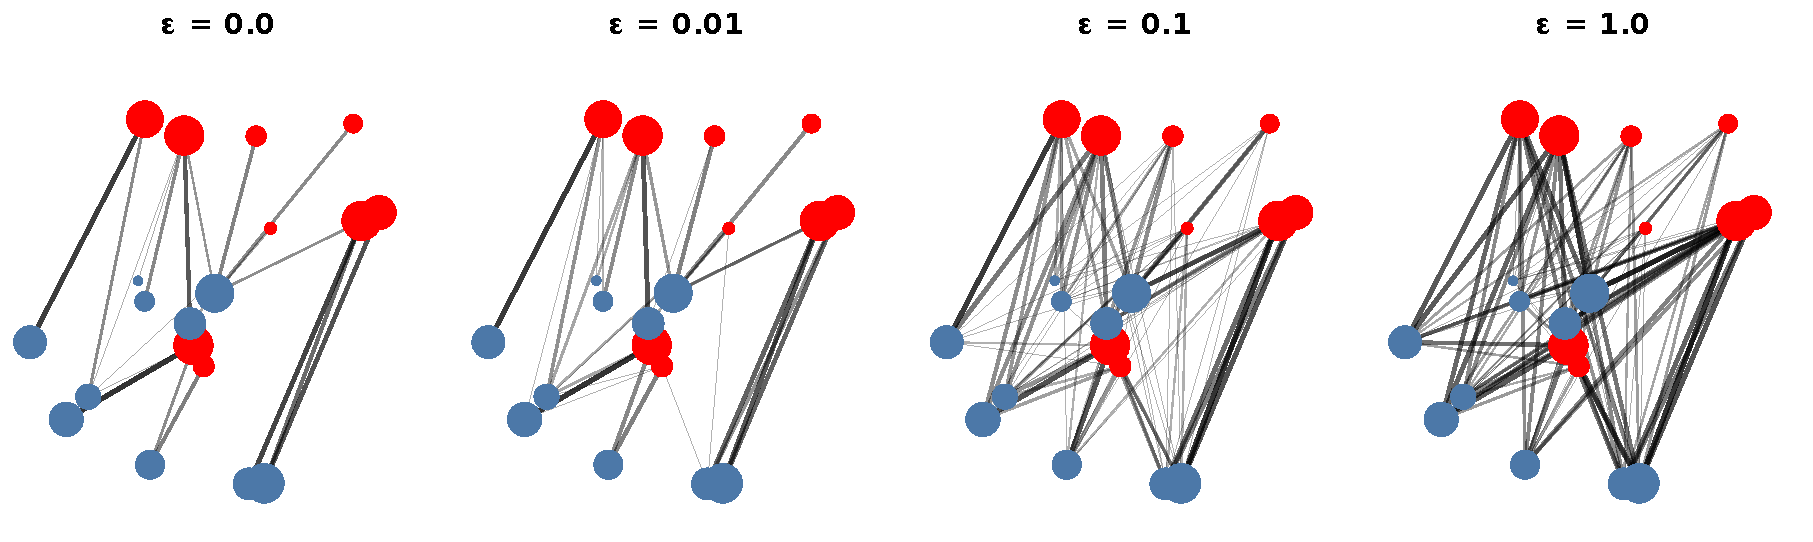
\includegraphics[width=0.8\textwidth]{./figures/figure}
	\caption{Figure}
	\label{fig:figure}
\end{figure}
 and
\begin{figure}[H]
	 \centering
	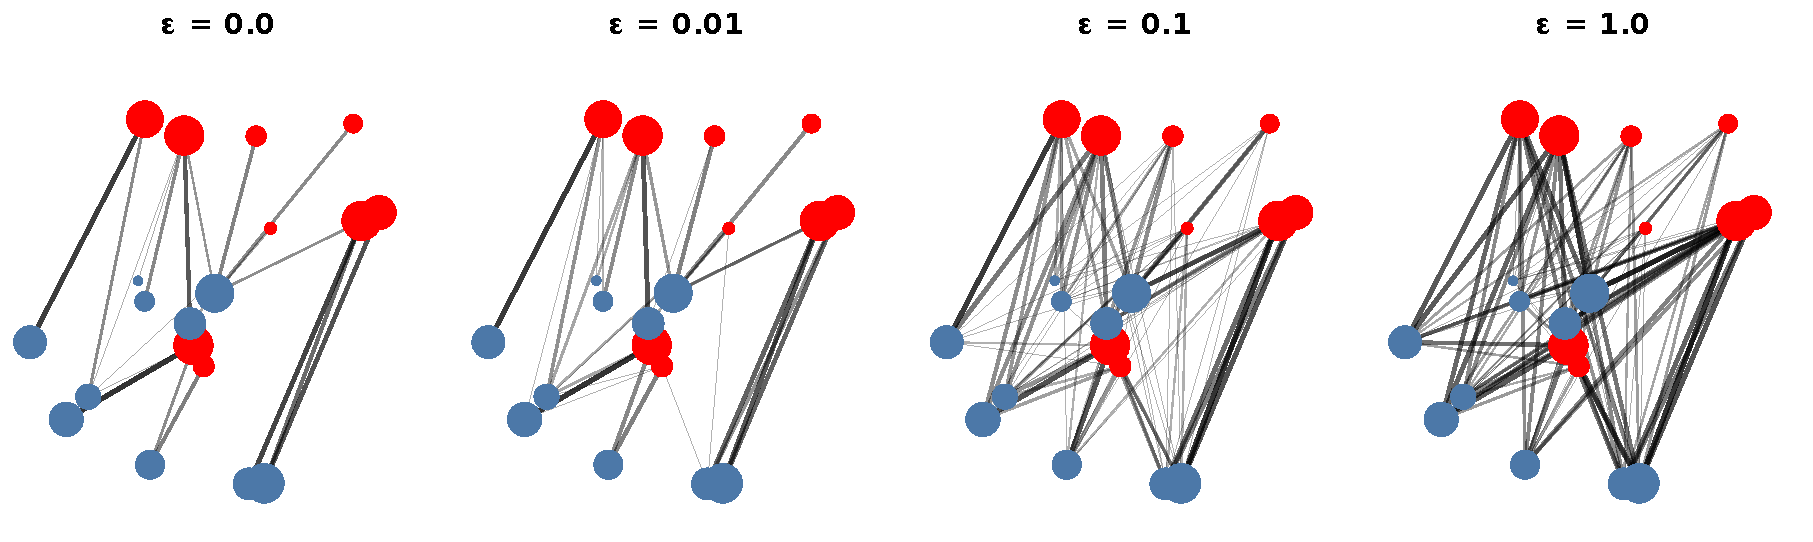
\includegraphics[width=0.8\textwidth]{./figures/figure}
	\caption{Figure 2}
	\label{fig:figure}
\end{figure}
 again.
\begin{lstlisting}[language=JuliaLocal, style=julia]
μ(x) = pdf(Normal(0,2),x)
println("Myplot")
Plots.plot(μ)
\end{lstlisting}

\begin{verbatim}
Myplot

\end{verbatim}

\begin{figure}[H]
	\centering
	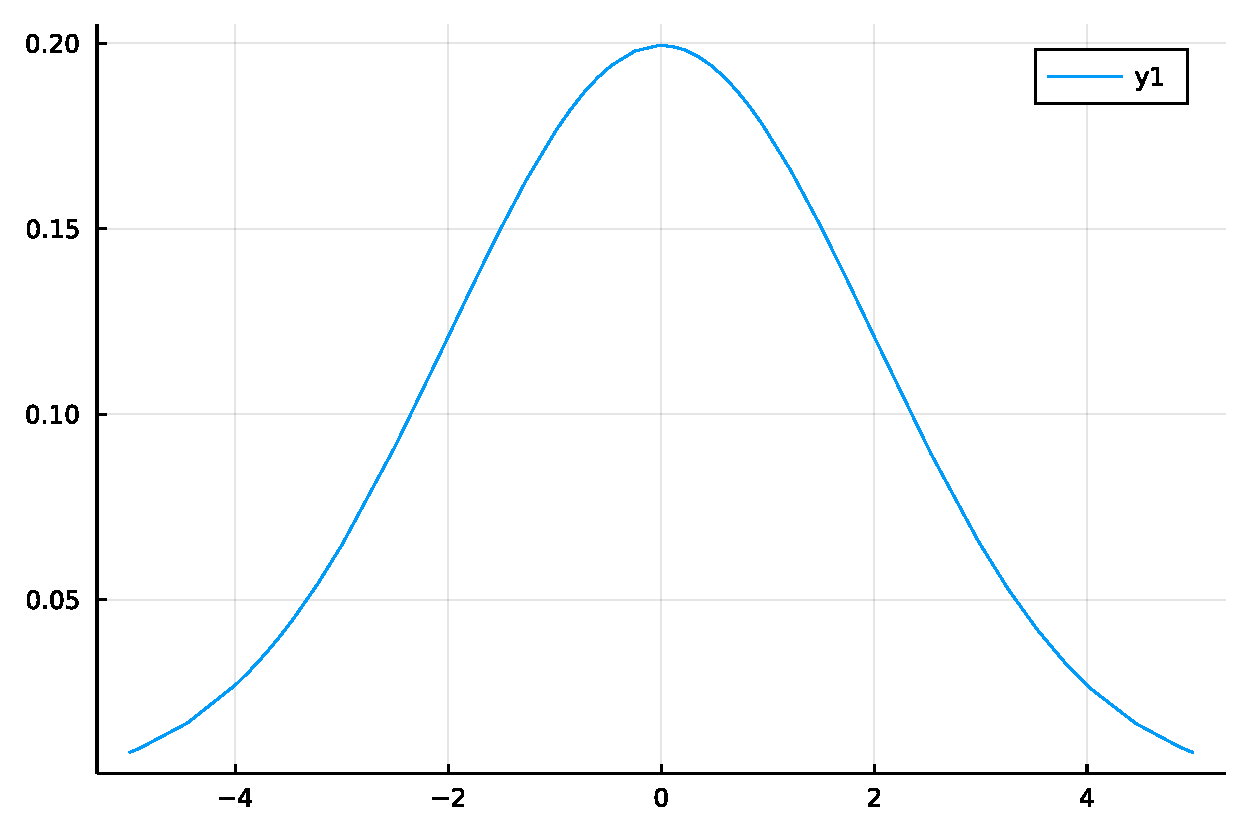
\includegraphics[width=0.8\textwidth]{./figures/jupyternotebook_figure1.pdf}
	\label{fig:jupyternotebook_figure1}

\end{figure}

\begin{lstlisting}[language=JuliaLocal, style=julia]
Makie.lines(-10:0.1:10, μ.(-10:0.1:10))
\end{lstlisting}

\begin{figure}[H]
	\centering
	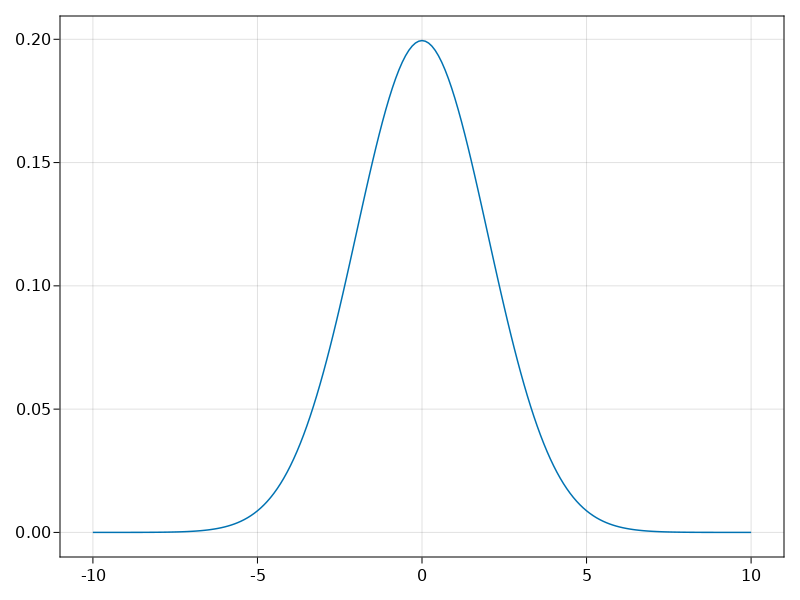
\includegraphics[width=0.8\textwidth]{./figures/jupyternotebook_figure2.png}
	\label{fig:jupyternotebook_figure2.png}

\end{figure}

\begin{lstlisting}[language=JuliaLocal, style=julia]
function example(μ)
    for i in 1:10
        println(μ(i))
    end
end
example(μ)
\end{lstlisting}

\begin{verbatim}
0.17603266338214976
0.12098536225957168
0.06475879783294587
0.02699548325659403
0.00876415024678427
0.0022159242059690038
0.0004363413475228801
6.691511288244268e-5
7.991870553452737e-6
7.433597573671488e-7

\end{verbatim}

\begin{verbatim}
0.17603266338214976
0.12098536225957168
0.06475879783294587
0.02699548325659403
0.00876415024678427
0.0022159242059690038
0.0004363413475228801
6.691511288244268e-5
7.991870553452737e-6
7.433597573671488e-7

\end{verbatim}

\begin{lstlisting}[language=JuliaLocal, style=julia]
rand(10)
\end{lstlisting}

\begin{figure}[H]
	 \centering
	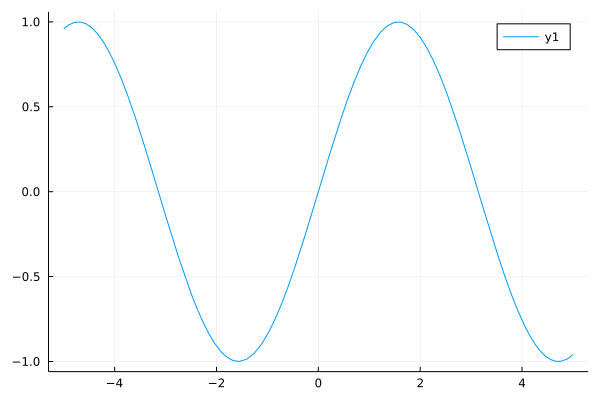
\includegraphics[width=0.8\textwidth]{./figures/plotexample.png}
	\caption{Figure2}
	\label{fig:plotexample.png}
\end{figure}
A raw cell
\begin{lstlisting}[language=JuliaLocal, style=julia]
DataFrame(x=rand(10),y=rand(10))
\end{lstlisting}

\begin{tabular}{r|cc}
	& x & y\\
	\hline
	& Float64 & Float64\\
	\hline
	1 & 0.0326174 & 0.589007 \\
	2 & 0.368715 & 0.690396 \\
	3 & 0.366451 & 0.803439 \\
	4 & 0.212434 & 0.581906 \\
	5 & 0.140433 & 0.678201 \\
	6 & 0.329857 & 0.50792 \\
	7 & 0.828484 & 0.0507595 \\
	8 & 0.480084 & 0.021381 \\
	9 & 0.784926 & 0.504361 \\
	10 & 0.43102 & 0.316321 \\
\end{tabular}
